
%%%%%%%%%%%%%%%%%%%%%%%%%%%%%%%%%%%%%%%%%%%%%%
\chapter{Анализ предметной области}
\section{Общие сведения о цифровых фильтрах}
Цифровой фильтр --- в электронике любой фильтр, обрабатывающий цифровой сигнал с целью выделения и/или подавления определённых частот этого сигнала. В отличие от цифрового, аналоговый фильтр имеет дело с аналоговым сигналом, его свойства не дискретны, соответственно передаточная функция зависит от внутренних свойств составляющих его элементов.\cite{didfileters}

Цифровые фильтры на сегодняшний день применяются практически везде, где требуется обработка потоков сигналов, приходящих с искусственных спутников Земли и др. В частности в спектральном анализе, обработке изображений, обработке видео, обработке речи и звука и многих других приложениях.

Несмотря на то, что цифровые фильтры могут быть нелинейными и нестационарными, наибольшее распространение получили линейные стационарные фильтры в силу простоты их поведения и математического описания. Линейность фильтра подразумевает, что если подать на вход арифметическую сумму отсчётов некоторых сигналов, то на выходе фильтра будет арифметическая сумма откликов фильтра на эти сигналы. Основными характеристиками стационарных линейных дискретных фильтров являются следующие:

\begin{itemize}
	\item импульсная характеристика;
	\item комплексная частотная характеристика;
	\item амплитудно-частотная и фазочастотная характеристики;
	\item системная функция (передаточная функция).	
\end{itemize}

Импульсной характеристикой дискретного фильтра называется его реакция на единичный импульс при нулевых начальных условиях. Линейный стационарный цифровой фильтр характеризуется передаточной функцией. Передаточная функция может описать, как фильтр будет реагировать на входной сигнал. Таким образом, проектирование фильтра состоит из постановки задачи (например, фильтр восьмого порядка, фильтр нижних частот с конкретной частотой среза), а затем производится расчет передаточной функции, которая определяет характеристики фильтра \cite{easyguide}.

Передаточная функция \footnote{Пeрeдаточная функция --- один из способов математического описания динамической системы. Используется в основном в теории управления, связи и цифровой обработке сигналов. Представляет собой дифференциальный оператор, выражающий связь между входом и выходом линейной стационарной системы. Зная входной сигнал системы и передаточную функцию, можно восстановить выходной сигнал.} фильтра имеет вид:
\begin{equation}
	H(z) = \frac{B(z)}{A(z)}  = \frac{{b_{0}+b_{1}z^{-1}+b_{2}z^{-2} + \cdots + b_{N}z^{-N}}}{{1+a_{1}z^{-1}+a_{2}z^{-2} + \cdots +a_{M}z^{-M}}}
\end{equation}

\section{Классификация шумов}
Шумы можно классифицировать по основным аспектам \cite{noise1}. К таким аспектам можно отнести следующие:
\begin{enumerate}
	\item Спектр.
		\begin{enumerate}
			\item Стационарные шумы.
			
			Стационарный шум --- шум, который характеризуется постоянством средних параметров: интенсивности (мощности), распределения интенсивности по спектру (спектральная плотность), автокорреляционной функции.
			
			Практически наблюдаемый шум, возникающий в результате действия многих отдельных независимых источников (например, шум толпы людей, моря, производственных станков, шум вихревого воздушного потока, шум на выходе радиоприёмника и др.), является квазистационарным.
			
			Классической моделью стационарного шума является белый шум.
			
			\item Нестационарные шумы.
			
			Нестационарный шум --- шум, длящийся короткие промежутки времени (меньшие, чем время усреднения в измерителях). Подразделяется на колеблющийся, прерывистый, импульсный.
			
			К нестационарным шумам относятся, например, уличный шум проходящего транспорта, отдельные стуки в производственных условиях, редкие импульсные помехи в радиотехнике и т. п.					
		\end{enumerate}
	
	\item Характер спектра.
		\begin{enumerate}
			\item Широкополосный шум с непрерывным спектром шириной более 1 октавы.
			\item Тональный шум, в спектре которого имеются выраженные тона. Выраженным тон считается, если одна из третьоктавных полос частот превышает остальные не менее, чем на 10 дБ.								
		\end{enumerate}
	

	
	\item Частота.
		\begin{enumerate}
			\item Низкочастотные (<300 Гц).
			\item Среднечастотные (300--800 Гц).
			\item Высокочастотные (>800 Гц).					
		\end{enumerate}
	
	\item Временные характеристики.
		\begin{enumerate}
			\item Стационарные.
			\item Нестационарные.
				\begin{enumerate}
					\item Колеблющиеся.
					\item Прерывистые.
					\item Импульсные.				
				\end{enumerate}
		
		\end{enumerate}
	
	\item Природа возникновения 
		\begin{enumerate}
			\item Механические.
			\item Аэродинамические.
			\item Гидравлические.
			\item Электромагнитные. 				
		\end{enumerate}
	
	\newpage
	
	\item Отдельные виды шумов \cite{noise2}.
		\begin{enumerate}
			\item Белый шум --- стационарный шум, спектральные составляющие которого равномерно распределены по всему диапазону задействованных частот.
			\item Цветные шумы --- некоторые виды шумовых сигналов, которые имеют определённые цвета, исходя из аналогии между спектральной плотностью сигнала произвольной природы и спектрами различных цветов видимого света.
			\item Розовый шум --- (в строительной акустике), у которого уровень звукового давления изменяется в октавной полосе частот.				
		\end{enumerate}	

	\item Неакустические шумы.
		\begin{enumerate}
			\item Радиоэлектронные шумы --- случайные колебания токов и напряжений в радиоэлектронных устройствах, возникают в результате неравномерной эмиссии электронов в электровакуумных приборах (дробовой шум, фликкер-шум), неравномерности процессов генерации и рекомбинации носителей заряда (электронов проводимости и дырок) в полупроводниковых приборах, теплового движения носителей тока в проводниках (тепловой шум).
			\item Тепловое излучение Земли и земной атмосферы, а также планет, Солнца, звёзд, межзвёздной среды и т. д. (шумы космоса).
			\item На Земле также имеются необъяснимые шумовые явления (звуковые аномалии).
		\end{enumerate}
\end{enumerate}

Таким образом, можно сделать вывод о том, что в реальной жизни не существует сигналов без шумов, а источников помех --- огромное количество. Безусловно, многие из них могут быть минимизированны аппаратными способами, однако не всегда целесообразно. Именно поэтому почти всегда наряду с базовыми аппаратными защитами используются методы программной фильтрации в цифровых фильтрах. Приведенные далее алгоритмы направленны на ликвидацию двух видов шума: белый шум с относительно стабильной амплитудой и случайные импульсы, вызванные внешними факторами. \cite{usage}
%%%%%%%%%%%%%%%%%%%%%%%%%%%%%%%%%%%%%%%%%%%%%%
\chapter{Классификация существующих методов}

\section{Методы фильтрации сигналов}
Далее представлены основные методы фильтрации сигналов. Описаны их принципы работы и определены краткие характеристики. \cite{theorysignal}

В качестве примеров для фильтрации будут рассмотрены следующие сигналы: синусоида, квадратный сигнал (дискретный или цифровой) и треугольный сигнал (рисунок \ref{img_1}). 

\begin{figure}[h]
	\begin{center}
		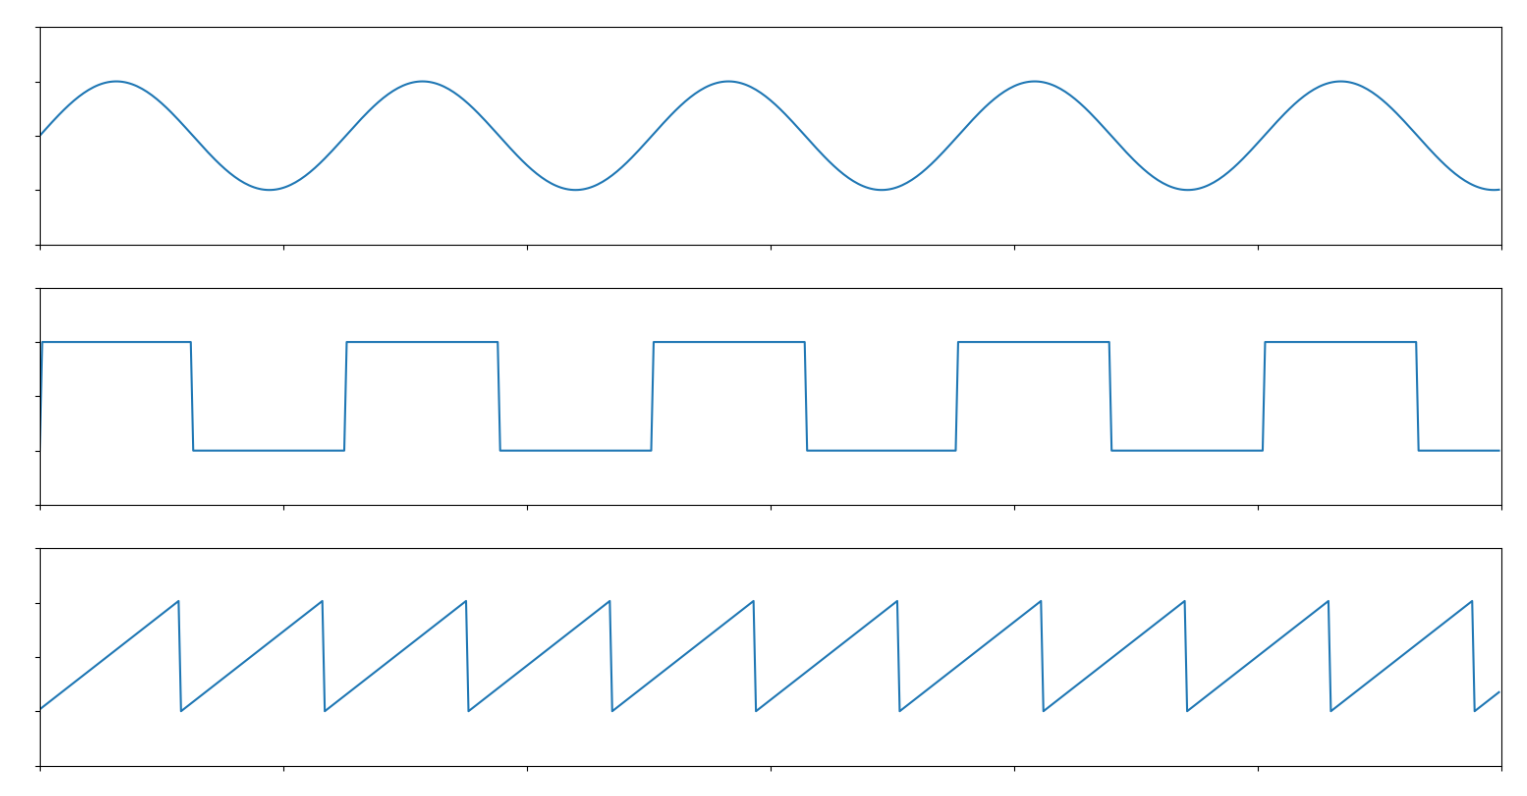
\includegraphics[pages=-, scale=0.22]{./inc/img/1.png}
		\caption{Чистые сигналы без помех (сверху вниз): синусоида, квадратный и треугольный}  
		\label{img_1}
	\end{center}
\end{figure}

Также будут рассмотрены указанные выше сигналы с шумами (рисунок \ref{img_2}).

\begin{figure}[h]
	\begin{center}
		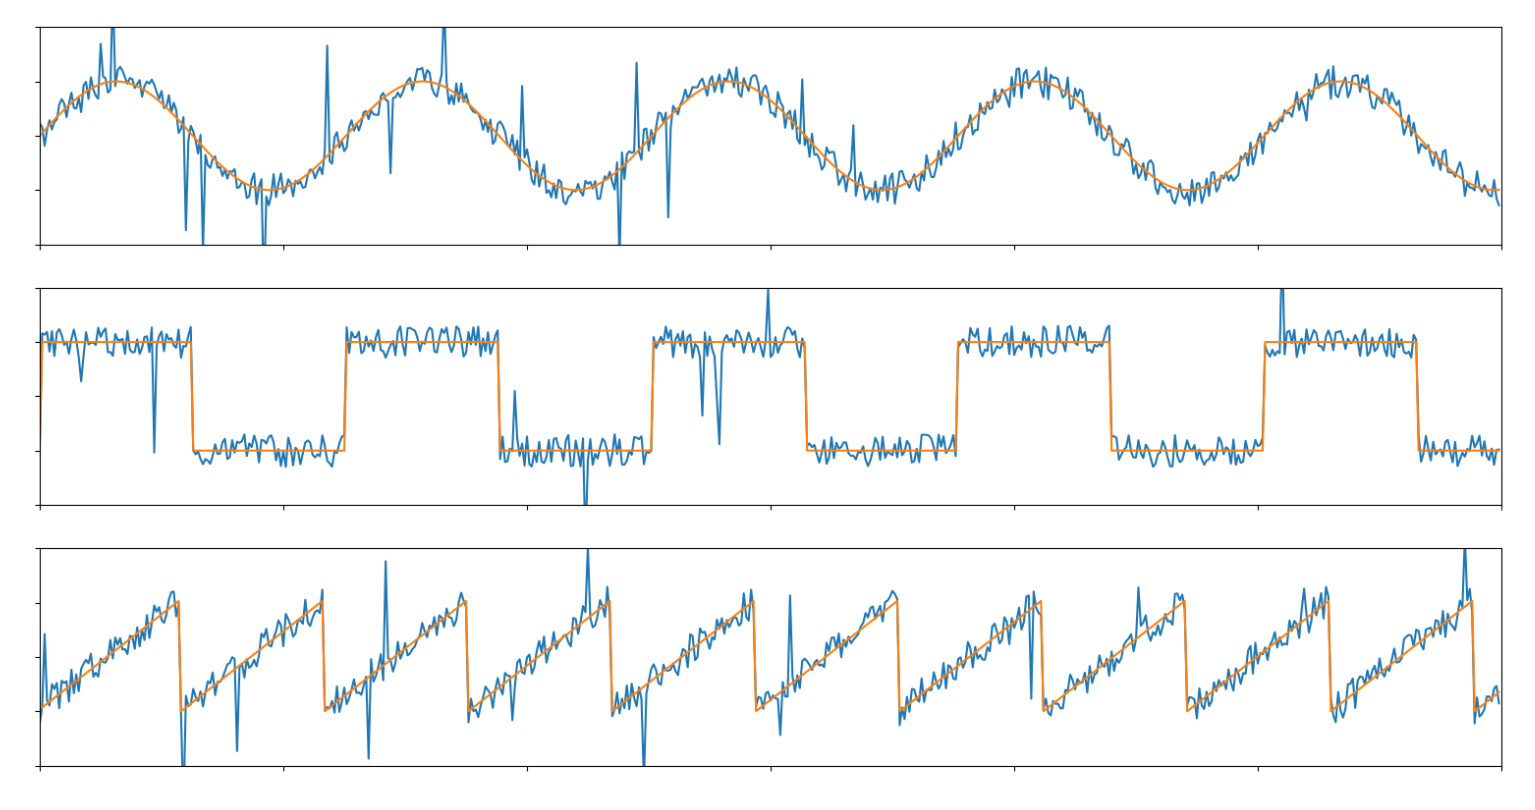
\includegraphics[pages=-, scale=0.22]{./inc/img/2.png}
		\caption{Cигналы с шумами (сверху вниз): синусоида, квадратный и треугольный}  
		\label{img_2}
	\end{center}
\end{figure}

\newpage

\subsection{Метод среднего арифметического}

Разностное уравнение\footnote{Разностное уравнение --- уравнение, связывающее значение некоторой неизвестной функции в любой точке с её значением в одной или нескольких точках, отстоящих от данной на определенный интервал. Применяется для описания дискретных систем.}, которое характеризует фильтр среднего арифметического, является уравнением КИХ-фильтра\footnote{Фильтр с конечной импульсной характеристикой — один из видов линейных цифровых фильтров, характерной особенностью которого является ограниченность по времени его импульсной характеристики (с какого-то момента времени она становится точно равной нулю). Такой фильтр называют ещё нерекурсивным из-за отсутствия обратной связи. Знаменатель передаточной функции такого фильтра --- константа.}. \cite{avg1}

Пусть $x_n$ --- входной сигнал фильтра, $y_n$ --- выходной сигнал, $P$ --- порядок фильтра, $b_i$ --- весовые коэффициенты отсчётов. Тогда разностное уравнение будет иметь вид:
\begin{equation}
	y_n = \sum_{i=0}^{P} b_i x_{n-i}
\end{equation}

Отличительной особенностью фильтра скользящего среднего является равенство единице суммы коэффициентов $b_i$:

\begin{equation}
	\sum_{i=0}^{P} b_i = 1
\end{equation}
	
Последнее выражение нормировки коэффициентов отличает скользящее среднее от других КИХ-фильтров. В частности, для простого скользящего среднего весовые коэффициенты отсчётов имеют следующий вид:

\begin{equation}
	b_{i}=\frac{1}{P+1} 
\end{equation}
для $i=0,1,\dots,P$.

Для реализации потребуется ввести буфер нескольких предыдущих значений, каждый раз, когда опрашивается датчик, буфер сдвигается (первый элемент удаляется, а новое значение датчика добавляется в конец или как-нибудь по другому, главное фиксированный размер буфера). От его размера и будет зависеть результат и быстродействие кода. С фильтрацией алгоритм справляется очень неплохо. Но его проблема заключается в производительности. Контроллеру приходится делать множество вычислений с плавающей точкой, что может сказаться на скорости выполнения кода. Но если датчик не следует очень часто опрашивать, то этот метод отлично подойдет.

\begin{figure}[h]
	\begin{center}
		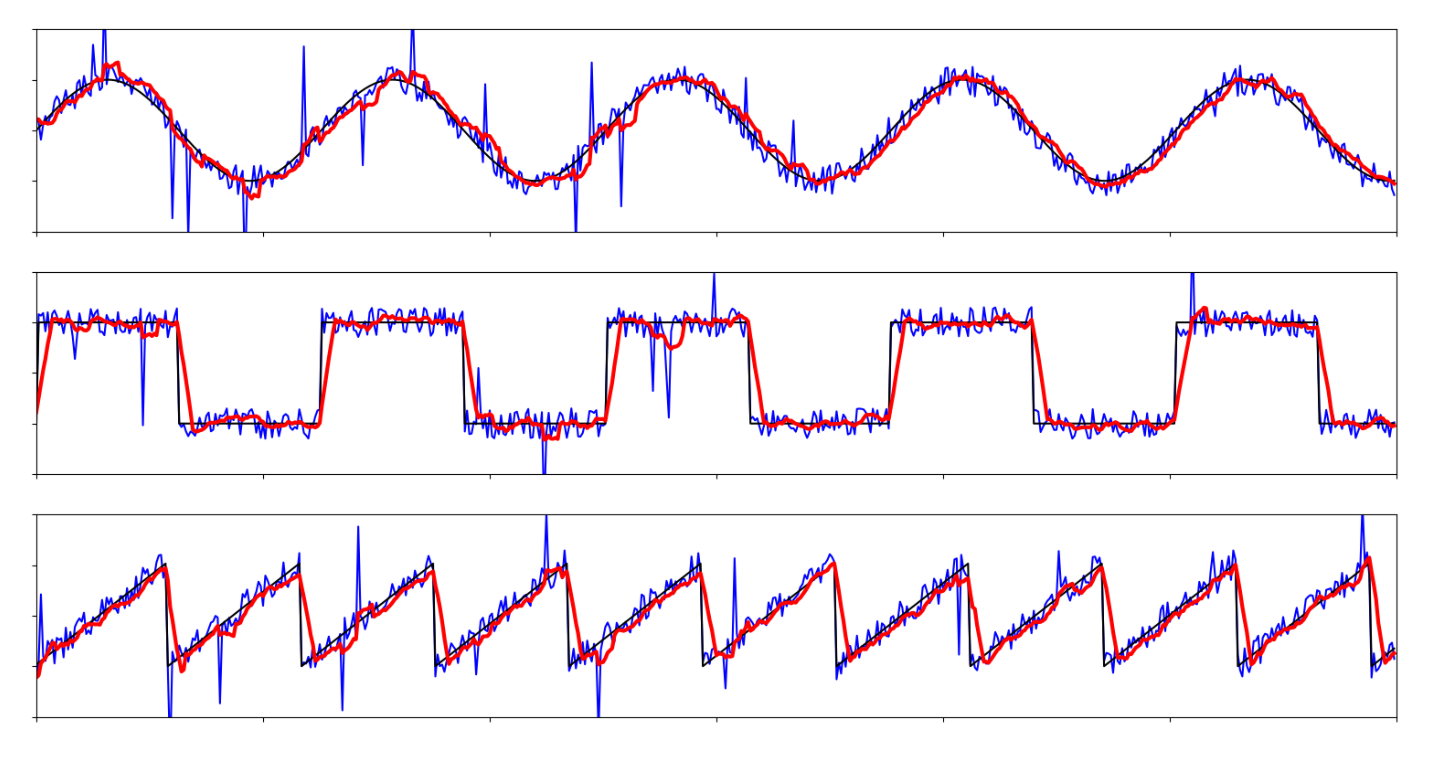
\includegraphics[pages=-, scale=0.32]{./inc/img/3.png}
		\caption{Фильтрация методом среднего арифметического, размер буфера = 7}  
		\label{img_3}
	\end{center}
\end{figure}

\begin{figure}[h]
	\begin{center}
		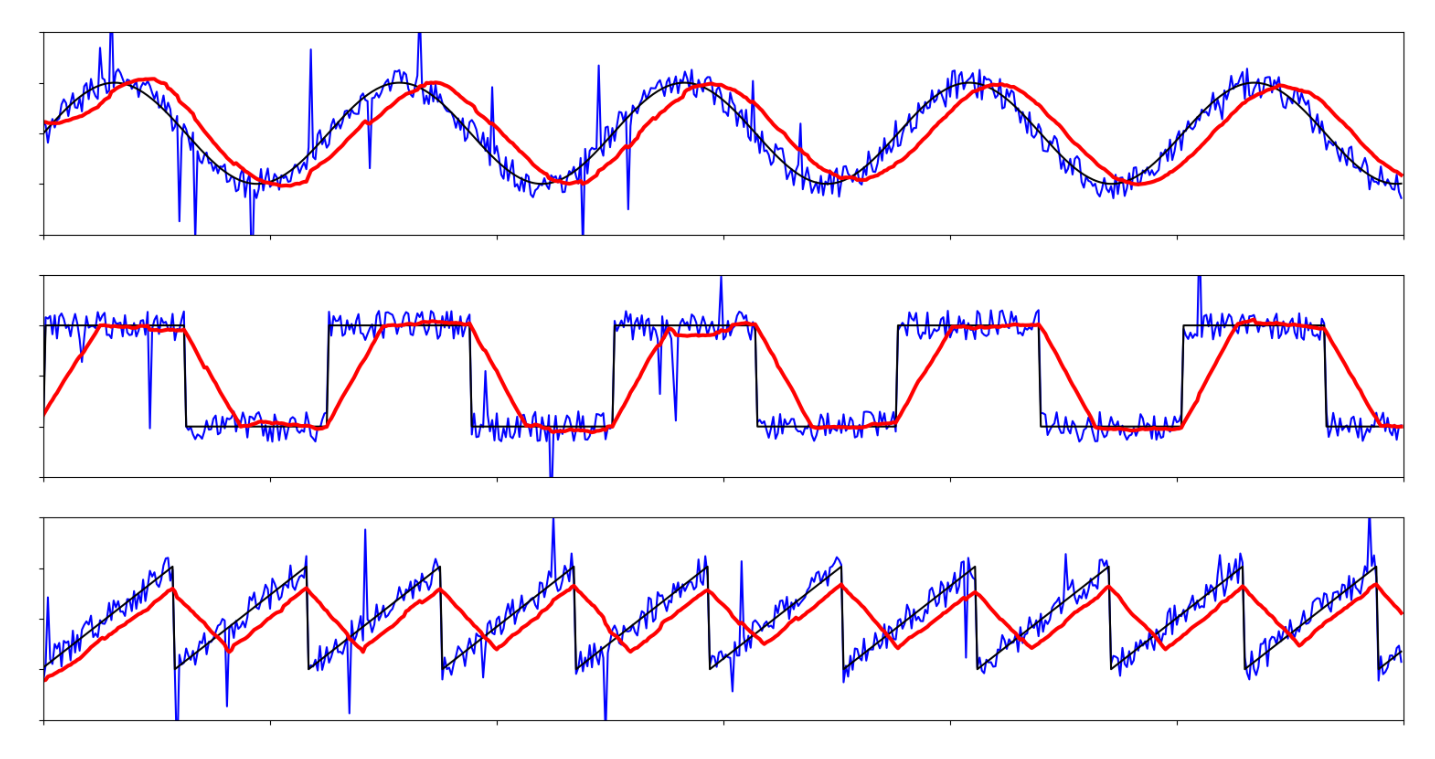
\includegraphics[pages=-, scale=0.32]{./inc/img/4.png}
		\caption{Фильтрация методом среднего арифметического, размер буфера = 25}  
		\label{img_4}
	\end{center}
\end{figure}

Исходя из рисунков \ref{img_3}--\ref{img_4}, можно сделать вывод о том, что при увеличении буфера квадратный и треугольный сигналы сильно исказились, а синусоида сместилась. Проявляется запаздывание среднего значения. Таким образом, при использовании данного фильтра следует аккуратно подбирать размер буфера.

\newpage


\subsection{Метод медианной фильтрации}

Медианная фильтрация --- эффективная процедура обработки сигналов, подверженных воздействию импульсных помех. \cite{med1}

Медианный фильтр $M$ из входящего сигнала $C$ создаёт медианный образ сигнала $\widetilde{C}$.
Входящий сигнал $C$ подаётся на медианный фильтр $M:C \rightarrow \widetilde{C}$.

В медианном фильтре сначала производится выбор значений, попавших в окно фильтра при нахождении окна в точке $x$, $\hat{O}(x):C \rightarrow O$.

Далее производится сортировка значений окна $O$ функцией сравнения значений $\Phi$ и строится упорядоченное множество $\Phi(O) \rightarrow \widetilde{O}$, а после выбирается медианное значение\footnote{Медиана набора чисел --- число, которое находится в середине этого набора, если его упорядочить по возрастанию, то есть такое число, что половина из элементов набора не меньше него, а другая половина не больше}: $m(\widetilde{O}) \rightarrow o_{m}$ и записывается в $\widetilde{C}(x)= o_{m}$.

Таким образом, медианный фильтр $M:C \rightarrow \widetilde{C}$ является последовательностью трёх действий:
\begin{enumerate}
	\item Выбор значений, попавших в окно фильтра $\hat{O}(x):C \rightarrow O$.
	\item Сортировка значений окна $\Phi(O) \rightarrow \widetilde{O}$.
	\item Выбор из $\widetilde{O}$ медианного значения $m(\widetilde{O}) \rightarrow o_{m}$ и запись его в медианный образ сигнала $\widetilde{C}$ в точку с координатой $x$, $\widetilde{C}(x) = o_{m} $.
\end{enumerate}
Эти действия повторяются для каждой точки входящего сигнала. \cite{med2}

Ниже приведен, пример реализации медианной функции. Следует отметить, что подобная реализация медианного фильтра станет бесполезной, если ширина импульсов будет больше единицы дискретизации\footnote{Единица дискретизации --- частота взятия отсчётов непрерывного по времени сигнала при его дискретизации (в частности, аналого-цифровым преобразователем). Измеряется в герцах. Чем выше частота дискретизации, тем более широкий спектр сигнала может быть представлен в дискретном сигнале. Как следует из теоремы Котельникова, для того, чтобы однозначно восстановить исходный сигнал, частота дискретизации должна более чем в два раза превышать наибольшую частоту в спектре сигнала.}.

\begin{equation}
	M = 
	\begin{cases}
		max(a, c), &\text{если $max(a, b) = max(b, c)$}\\
		max(b, min(a, c) &\text{иначе}
	\end{cases}
\end{equation}

Медианный фильтр справляется почти со всеми импульсами. К тому же этот алгоритм совершенно прост в вычислении. И используя его в комбинации с каким-либо другим фильтром можно получить результат, максимально приближенный к требуемому.

\begin{figure}[h]
	\begin{center}
		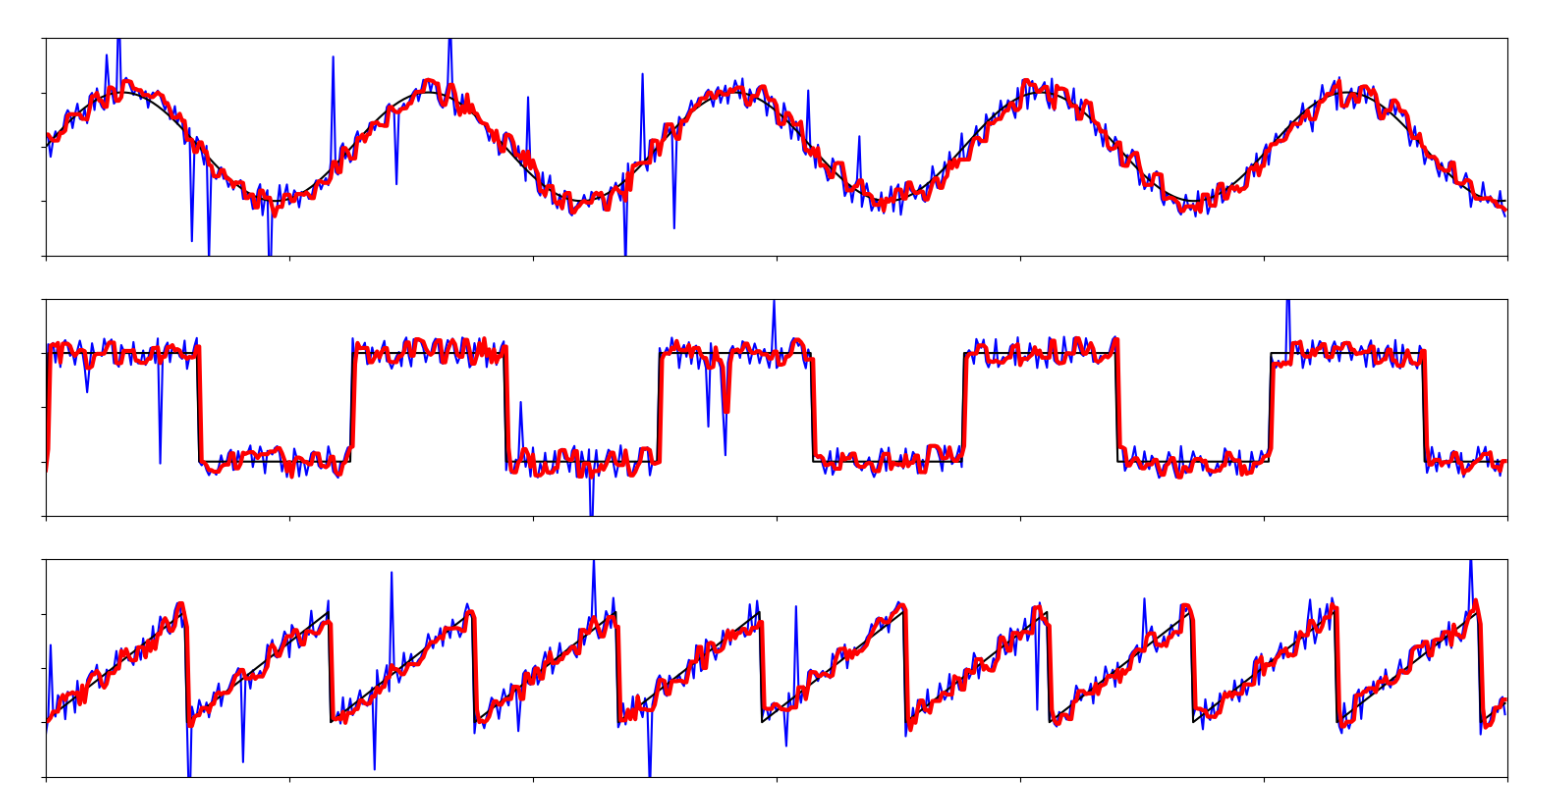
\includegraphics[pages=-, scale=0.32]{./inc/img/5.png}
		\caption{Медианная фильтрация сигналов}  
		\label{img_5}
	\end{center}
\end{figure}

\subsection{Экспоненциальное бегущее среднее и адаптивный коэффициент}

Экспоненциально взвешенное скользящее среднее --- разновидность взвешенной скользящей средней, веса которой убывают экспоненциально и никогда не равны нулю. \cite{glide1} Определяется следующей формулой

\begin{equation}
	\textit{EMA}_t  = \alpha \cdot p_t + (1-\alpha) \cdot \textit{EMA}_{t-1},
\end{equation}

где $\textit{EMA}_t$ --- значение экспоненциального скользящего среднего в точке $t$ (последнее значение, в случае временного ряда), $\textit{EMA}_{t-1}$ --- значение экспоненциального скользящего среднего в точке $t-1$ (предыдущее значение в случае временного ряда), $p_t$ --- значение исходной функции в момент времени $t$ (последнее значение, в случае временного ряда),
$\alpha$ ---  коэффициент характеризующий скорость уменьшения весов, принимает значение от 0 и до 1, чем меньше его значение тем больше влияние предыдущих значений на текущую величину среднего. \cite{diskretiz}

Первое значение экспоненциального скользящего среднего, обычно принимается равным первому значению исходной функции:
\begin{equation}
	\textit{EMA}_0  = p_0.
\end{equation}

Коэффициент $\ \alpha$, может быть выбран произвольным образом, в пределах от 0 до 1. \cite{med3} Например, он может быть выражен через величину окна усреднения:
\begin{equation}
	\ \alpha = \frac{2}{n + 1}.
\end{equation}

Этот фильтр по своей сути схож с первым, а главное он более простой по вычислениям. \cite{glide2} Работает он так: к предыдущему фильтрованному значению прибавляется новое, и каждое из них помножено на собственный коэффициент, сумма которых равна 1. Коэффициент k подбирается от 0 до 1 и означает важность нового значения по сравнению с предыдущим, то есть чем больше k, тем больше важность нового нефильтрованного значения и фильтрованный график ближе к изначальному. \cite{med4}

\begin{equation}
	normalised += (new - normalised) * k
\end{equation}

Адаптивный коэффициент нужен для корректной фильтрации квадратных сигналов:

\begin{equation}
	k = 
	\begin{cases}
		s_k, &\text{если $|new - normalised| < d$}\\
		max_k &\text{иначе}
	\end{cases}
\end{equation}

Данная фильтрация работает с достаточно высокой точностью, но из-за адаптивного коэффициента появляются некие артефакты в моментах с импульсами (рисунок \ref{img_6}), так как они достаточно велики, чтобы определиться как составляющие квадратного сигнала. Это можно нивелировать, увеличивая параметр d (требуемое расстояние для определения квадратного сигнала). В то же время можно воспользоваться медианным фильтром. Если перед подачей данных на бегущее среднее применить медианную фильтрацию \cite{glide3}, то возможно исправить нежелательные артефакты (рисунок \ref{img_7}).


\newpage

\begin{figure}[h]
	\begin{center}
		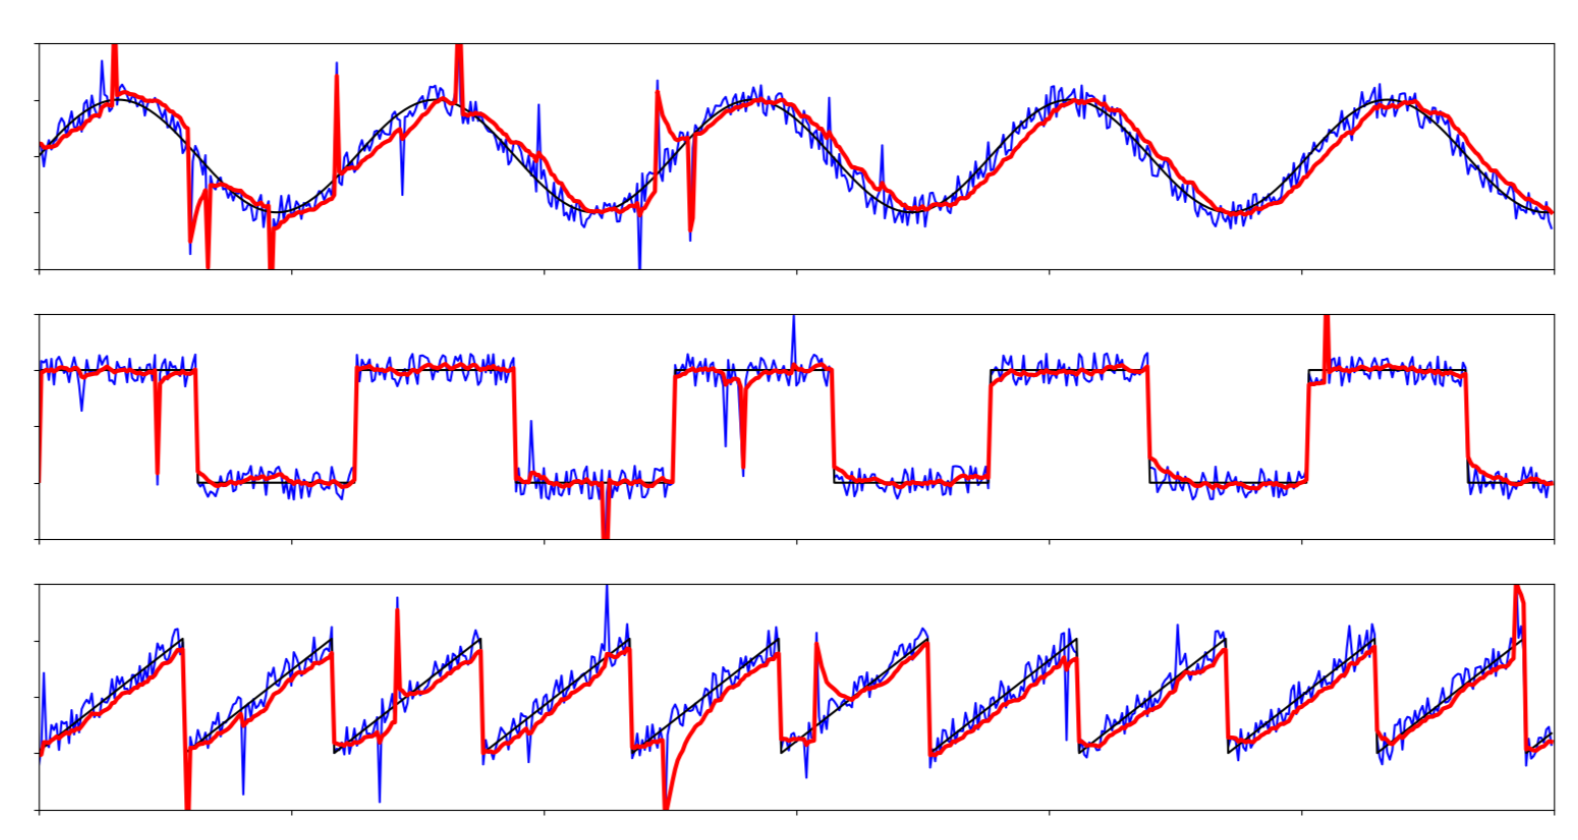
\includegraphics[pages=-, scale=0.33]{./inc/img/6.png}
		\caption{Фильтрация с использованием экспоненциального бегущего среднего и адаптивного коэффициента}  
		\label{img_6}
	\end{center}
\end{figure}

\begin{figure}[h]
	\begin{center}
		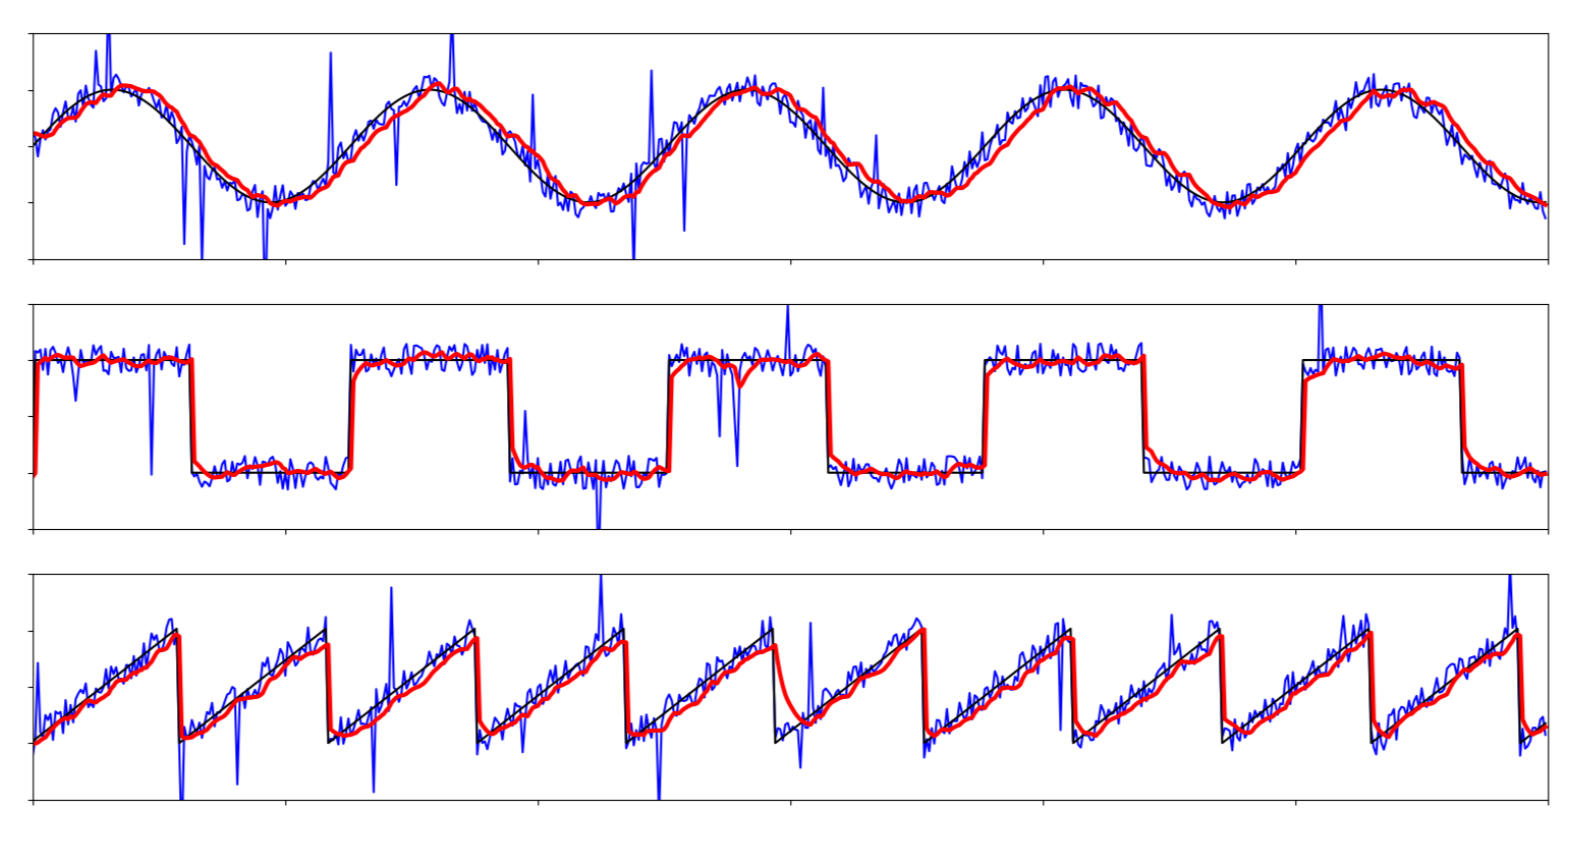
\includegraphics[pages=-, scale=0.33]{./inc/img/7.png}
		\caption{Фильтрация с использованием экспоненциального бегущего среднего и адаптивного коэффициента в связке с медианной фильтрацией}  
		\label{img_7}
	\end{center}
\end{figure}

Данная связка алгоритмов является одной из самых эффективных и быстродейственных. Она может быть применена для сигнала любой природы и сложности, при этом показывая качественный результат.

\newpage

\subsection{Фильтр Калмана}

Фильтр Калмана --- эффективный рекурсивный фильтр\footnote{ Рекурсивный фильтр --- линейный электронный фильтр, использующий один или более своих выходов в качестве входа, то есть образующий обратную связь. Основным свойством таких фильтров является то, что их импульсная переходная характеристика имеет бесконечную длину во временной области, а передаточная функция имеет дробно-рациональный вид.}, оценивающий вектор состояния динамической системы, используя ряд неполных и зашумленных измерений. \cite{calman1}

Фильтр Калмана оперирует понятием вектора состояния системы (набором параметров, описывающих состояние системы на некоторый момент времени) и его статистическим описанием. В общем случае динамика некоторого вектора состояния описывается плотностями вероятности распределения его компонент в каждый момент времени. При наличии определённой математической модели производимых наблюдений за системой, а также модели априорного изменения параметров вектора состояния (а именно --- в качестве марковского формирующего процесса) можно записать уравнение для апостериорной плотности вероятности вектора состояния в любой момент времени. Данное дифференциальное уравнение носит название уравнение Стратоновича. Уравнение Стратоновича в общем виде не решается. Аналитическое решение удается получить только в случае ряда ограничений (предположений):
\begin{itemize}
	\item гауссовые априорные и апостериорные плотности вероятности вектора состояния на любой момент времени (в том числе начальный);
	\item гауссовые формирующие шумы;
	\item гауссовые шумы наблюдений;
	\item белые шумы наблюдений;
	\item линейность модели наблюдений;
	\item линейность модели формирующего процесса (который должен являться марковским процессом).
\end{itemize}

Классический фильтр Калмана является уравнениями для расчета первого и второго момента апостериорной плотности вероятности (в смысле вектора математических ожиданий и матрицы дисперсий, в том числе взаимных) при данных ограничениях. Ввиду того, что для нормальной плотности вероятности математическое ожидание и дисперсионная матрица полностью задают плотность вероятности, можно сказать, что фильтр Калмана рассчитывает апостериорную плотность вероятности вектора состояния на каждый момент времени. А значит полностью описывает вектор состояния как случайную векторную величину.

Расчетные значения математических ожиданий при этом являются оптимальными оценками по критерию среднеквадратической ошибки, что и обуславливает его широкое применение.

При использовании фильтра Калмана для получения оценок вектора состояния процесса по серии зашумленных измерений необходимо представить модель данного процесса в соответствии со структурой фильтра --- в виде матричного уравнения определённого типа. Для каждого такта $k$ работы фильтра необходимо в соответствии с приведенным ниже описанием определить матрицы: эволюции процесса $F_k$; матрицу наблюдений $H_k$; ковариационную матрицу процесса $Q_k$; ковариационную матрицу шума измерений $R_k$; при наличии управляющих воздействий --- матрицу их коэффициентов $B_k$. \cite{calman2}

Модель системы/процесса подразумевает, что истинное состояние в момент $k$ получается из истинного состояния в момент $k-1$ в соответствии с уравнением:
\begin{equation}
	x_{k} = {F}_{k} {x}_{k-1} + {B}_{k} {u}_{k} + {w}_{k},
\end{equation}
где $F_k$ — матрица эволюции процесса/системы, которая воздействует на вектор $x_{k-1}$ (вектор состояния в момент $k-1$), $B_k$ — матрица управления, которая прикладывается к вектору управляющих воздействий $u_k$, $w_k$ — нормальный случайный процесс с нулевым математическим ожиданием и ковариационной матрицей $Q_k$, который описывает случайный характер эволюции системы:
\begin{equation}
	 {w}_{k} \sim N(0, {Q}_k)
\end{equation}

В момент $k$ производится наблюдение (измерение) $z_k$ истинного вектора состояния $x_k$, которые связаны между собой уравнением:
\begin{equation}
	{z}_{k} = {H}_{k} {x}_{k} + {v}_{k} 
\end{equation}
где $H_k$ --- матрица измерений, связывающая истинный вектор состояния и вектор произведенных измерений, $v_k$ --- белый гауссовский шум измерений с нулевым математическим ожиданием и ковариационной матрицей $R_k$:
\begin{equation}
	{v}_{k} \sim N(0, {R}_k) 
\end{equation}

Начальное состояние и векторы случайных процессов на каждом такте считаются независимыми. \cite{calman3}

\begin{figure}[h]
	\begin{center}
		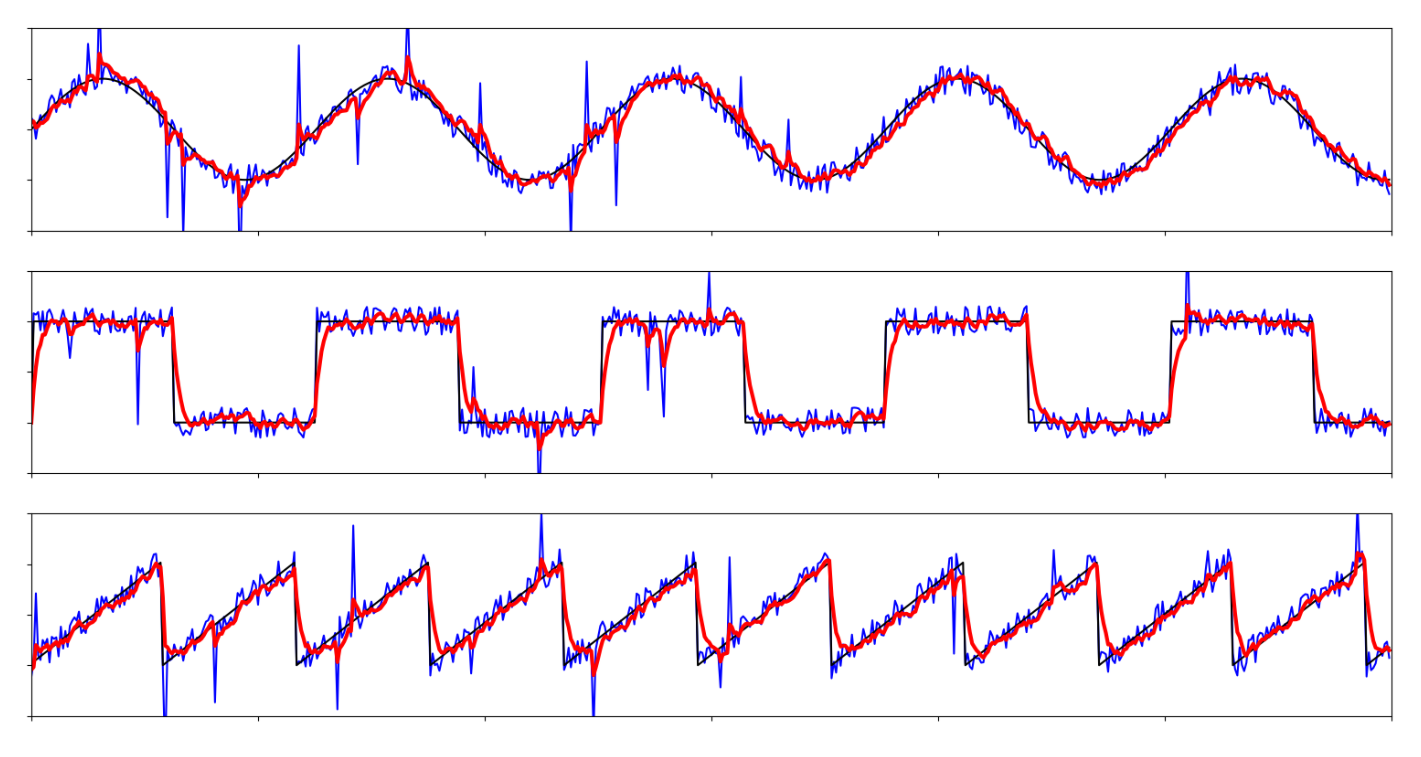
\includegraphics[pages=-, scale=0.40]{./inc/img/8.png}
		\caption{Фильтрация сигналов методом Калмана}  
		\label{img_8}
	\end{center}
\end{figure}

Стоить отметить, что несмотря на высокую степень фильтрации и точность, данный алгоритм имеет высокую вычислительную сложность, поэтому он не подходит для систем фильтрации реального времени.

Таким образом, были рассмотрены основные методы фильтрации сигналов, каждый из которых имеет свои плюсы и минусы. Но стоит сказать, что на этом список методов фильтрации не исчерпывается, их существует большое количество, но принципы их работы строятся на основе приведенных выше методов.

\newpage

\section{Сравнительный анализ рассмотренных решений}

Исходя из ранее приведенных сведений, можно выделить следующее:
\begin{itemize}
	\item метод среднего арифметического ввиду своей вычислительной простоты, как следствие высокой отказоустойчивостью ввиду отсутствия большого количества компонентов, но довольно грубой степени фильтрации с ограничениями подходит для использования в качестве резервного в различных системах на случай выхода из строя основного цифрового фильтра;
	\item метод медианной фильтрации является наиболее предпочтительным в большинстве ситуаций ввиду своей низкой вычислительной сложности и высокого качества фильтрации. Также метод медианной фильтрации возможно сочетать с другими видами фильтраций для достижения наилучшего результата;
	\item метод фильтрации экспоненциального бегущего среднего и адаптивного коэффициента следует использовать следует использовать как дополнительный метод вторичной фильтрации;
	\item фильтрация Калмана является математически точным методом устранения шумов из сигналов, однако ощутимо растет вычислительная сложность, т.к. в ходе вычислений происходит огромное количество операций с числами с плавающей точкой, использования больших объемов дополнительной памяти для описания математических структур, а также вызовов различных непростых математических операторов и функций. Ввиду выше сказанного, данный метод не подходит для работы в системах фильтрации реального времени, таких как системы потоковой передачи видео, изображений и другого медиа, а также систем спутниковой навигации, но данный метод может себя отлично проявить при фильтрации архивных сигналов (например, улучшение качества звуковых сигналов переговоров лётчиков и диспетчеров во время авиакатастроф).
	
\end{itemize}





